\subsection{What is Pressure?}
While the Zeroth law of thermodynamics allows for the notion of "temperature" to be well defined, it isn't a particularly useful definition. While it can tell us that, macroscopically, "temperature is what you read from a thermometer", it is of interest to see how the phenomenon of temperature arises microscopically. For this, we will first introduce the notion of pressure\footnote{{\tt https://www.youtube.com/watch?v=a01QQZyl-\_I}}.

We will here define the pressure $P$ as:

\begin{equation}
    P = \frac{F}{A}
\end{equation}

Where $F$ is the force exerted over a certain area $A$. A good way to think about this might be if I have a gas of pressure $P$ contained in a box, that would tell you that if one of the walls of the box has area $A$, there is a perpendicular force of $PA$ being applied.\\

Just how does this help us define temperature? In order for us to connect the pieces, it will be helpful to figure out how the pressure of a gas arises from the microscopic properties of the gas. For this, let us consider a very simple scenario of a single molecule of gas bouncing back and forth in a 1-dimensional tube. This might seem like a strange place to start, but we will shortly see that this simple start leads to valuable information about more complicated scenarios! Note that the below derivation is mainly for your own understanding, and is not especially crucial for your success in Thermodynamics.

\begin{center}
    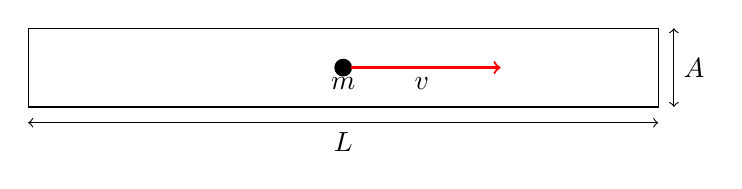
\begin{tikzpicture}[scale=4]
    \draw[draw=black] (0,0) rectangle(2,0.25);
    \filldraw (1,0.125) circle (0.75pt);
    \draw[red, ->, thick] (1.025,0.125) -- (1.5,0.125);
    \node[below] at (1,0.125) {$m$};
    \node[below] at (1.25,0.125) {$v$};
    \draw[<->] (0,-0.05) -- (2,-0.05);
    \draw[<->] (2.05,0) -- (2.05,0.25);
    \node[below] at (1,-0.05) {$L$};
    \node[right] at (2.05,0.125) {$A$};
    \end{tikzpicture}
\end{center}

Pictured above is our scenario; we have a single molecule of gas of mass $m$ and speed $v$ moving back and forth in a tube of length $L$, as it bounces off the ends of the tube that have area $A$. We assume that the molecule collides elastically off the walls, and hence it goes back and forth with velocities $\vec{v}$ and $-\vec{v}$. From our knowledge of kinematics, we obtain that the time it takes for the particle to go back and forth once is:
\begin{align*}
    \Delta t = \frac{2L}{v}
\end{align*}
Now, we want to figure out the average pressure that this particle applies on the wall; to obtain this, we, we return to how we have defined pressure above:
\begin{align*}
    P_{av} = \frac{F_{av}}{A}
\end{align*}
$A$ is just a constant here, so we then just need to figure out $F_{av}$! For this, we think back to the kinematics unit and the definition of force as the time derivative of momentum\footnote{Of course you know by know that force and momentum are vector and not scalar quantities, but since our problem is one dimensional, we can just consider the scalar version of the equation here!}:
\begin{align*}
    F = \frac{dp}{dt} = \frac{d(mv)}{dt}
\end{align*}
Since we are just concerned with the average force, we can just consider the change in momentum $\Delta p$ of the particle from hitting one of the ends over one cycle over the time it takes for one cycle (which is just $\Delta t$, above!). We consider that when the molecule hits the end of the tube with speed $v$, it reflects back elastically and starts going in the other direction with the same speed $v$, so its change in velocity is therefore $-2\Delta v$, and therefore the change in momentum is:
\[ \Delta p_{molecule} = -2m\Delta v\]
And therefore the average force applied to the wall is:
\[ F_{av} = \frac{-\Delta p_{molecule}}{\Delta t} = \frac{2mv}{\frac{2L}{v}} = \frac{mv^2}{L} \]
Then, getting the average pressure (from the one molecule) is simple, using the definition of pressure:
\[P_{av} = \frac{\frac{mv^2}{L}}{A} = \frac{mv^2}{V} \]
Where I have used the fact that the volume of the tube is given by $V = AL$. Now, in a real gas, we obviously don't just have one molecule, but a bunch of different molecules, all with different speeds! If we want the total pressure from a whole bunch of (say, $N$) molecules, we can just add up the average pressure of $N$ molecules:
\[P_{total} = \sum_{i=1}^N \frac{mv_i^2}{V}\]
As a reminder, the greek sigma $\Sigma$ above is telling us to take the "sum of N" things (in this case, molecules). It's clear that the volume can be taken out of the summation (because the volume of the tube is the same no matter which molecule we look at), and if we further assume that all of the masses of the molecules are the same (which is perfectly reasonable if we have a gas made of one element), then we obtain:
\[P_{total} = \frac{m}{V} \sum_{i=1}^N v_i^2 \]
Now I'm going to do a bit of a hack; I'm going to multiply this expression by $1 = \frac{N}{N}$:
\[P_{total} = N\frac{m}{V} \left(\frac{1}{N}\sum_{i=1}^N v_i^2 \right)\]
You might recognize from your physics labs that the quantity in brackets is just the \textit{average} of the squared velocities of all the molecules\footnote{To be clear, this is not the square of the averages!}; let us denote this by $v^2_{av}$. Now, let us multiply both sides by the volume $V$ of the box:
\[PV = Nmv^2_{av} \]
Now, if we multiply both sides by a half, we get something that looks familiar on the right hand side:
\[\frac{1}{2}PV = N\frac{1}{2}mv^2_{av} \]
You can see that we have exactly the average kinetic energy of our molecules (times the number of molecules in our system)! Now, at the beginning I said we were considering a one-dimensional system; but the direction we could have been talking about could have been the x direction, the y direction, or the z direction, and we would have got the same result! Therefore, we have that:
\[N\frac{1}{2}mv^2_{xav} = N\frac{1}{2}mv^2_{yav} = N\frac{1}{2}mv^2_{zav} = \frac{1}{2}PV \]
Therefore, for an ideal gas in three dimensions, all we have to do is add the three terms (the three kinetic energy contributions from each of the directions) together:
\begin{equation}
    \label{eqn:(2)}
    \frac{3}{2}PV = N\epsilon_{kavg}
\end{equation}
Where $\epsilon_{kavg}$ is the average kinetic energy of the molecules in three dimensions, defined as:
\begin{equation}
    \epsilon_{kavg} = \frac{1}{2}mv^2_{xav} + \frac{1}{2}mv^2_{yav} + \frac{1}{2}mv^2_{zav} = \frac{1}{2}m\vec{v}_{av} \cdot \vec{v}_{av}
\end{equation}
Now at this point, you might be holding your head in your hands because I spent three pages on a derivation\footnote{I sincerely apologize for your suffering.} and it seems like we're no closer to defining temperature than when we started. However, in the next section we will introduce the ideal gas law, and combining that with equation \ref{eqn:(2)} we just derived, we will see that we obtain exactly what we want to find. 